\chapter{Physics Background}
\section{The Phenomena of Spin}

Spin is a fundamental quantity possessed by all elementary particles. We use
the word 'spin' to describe the property, because partices which possess spin,
behave as though they have some kind of intrinsic, hidden rotation, as if they
were 'spinning'. The dimension of spin, therefore is angular momentum. What is
somewhat bizarre about spin, is that we do not observe anything physically
spinning - although there are some phenomena (such as oribtal angular momenta)
which can be naively thought of as a 'spinning system' (but this description
escapes classical analogy, due to its quantum, probibalistic nature). The role
of Spin in Physics is of foundational importance, and yet, we have not
succesfully produced a model which can accurately predict the spin of hadrons.

The presence of spin in relativistic particles creates the phenomona of
chriality, which has huge implications for how elementary particles can generate
structure in matter itself ~\needcite{}. In the case of the weak interaction,
the presence of spin, which creates Chiral spinors breaks the left-right
symmetry of weak coupling in matter (a fact which will be exploited in this
thesis to probe the spin of the proton sea).

The phenomena of spin also changes the rules for how ensembles of particles may
exist in a potential. Particles with spin are fermions, and because these
paritcles must obey fermi statistics, we can observe structure in matter in the
universe ~\needcite{}. Without spin, the world as we know would collapse on
itself, making any kind of extended non-exotic structures which currenlty exist
by virtue of the Pauli exclusion principal, impossible.

\clearpage
\section{A Brief History of Proton Spin}

The study of Spin is really just an outgrowth of the general study of matter.
Our models for matter, and the underlying structure of matter (in the modern
sense), represents over a hundred years of experimental and theoretical efforts,
and thousands of years of contemplating what makes up the universe.

Although indulgent on my part, I find it interesting, and humbling, to try and
map out the path that humanity and science has trodden on its way to
understanding the building blocks of the universe. To find the first time that
humanity had murmurings that suggested our visible world is built from
invisible, fundamental building blocks, we must travel back, nearly 2,500 years
into the past.

\subsection{Ancient Foundations}
Sometime around 490 - 370 BCE lived two philosophers, empedocles
(Fig~\ref{fig:empedocles}), and Democrtius (Fig~\ref{fig:democritus}). Both men
lived approximately at the same time, and made huge philosophical leaps in
attempting to understand the nature of the visible world.

\begin{figure}[ht]
	\centering
	\begin{subfigure}{.5\textwidth}
		\centering
		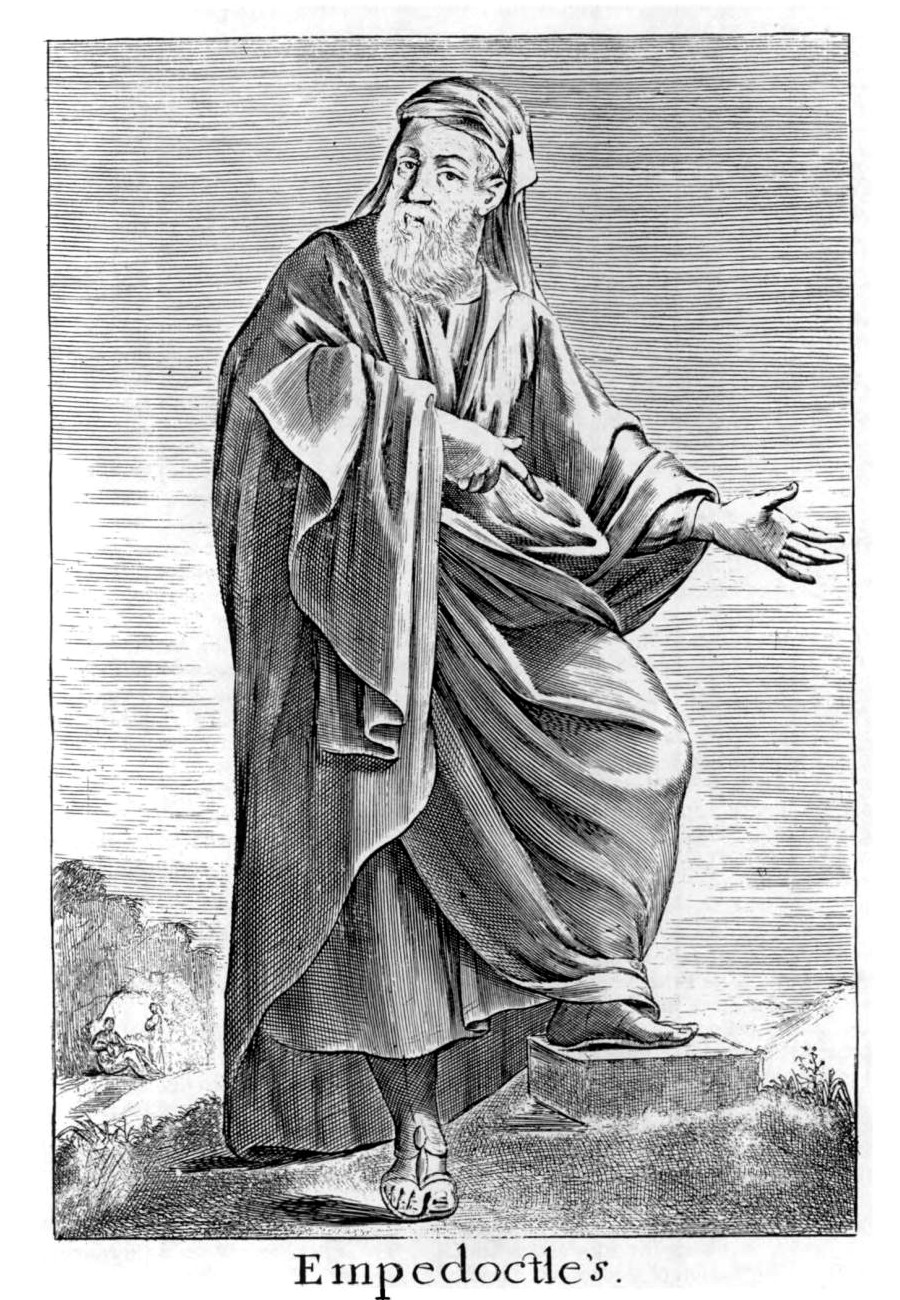
\includegraphics[width=0.4\linewidth]{../Chapter2/fig/empedocles.jpg}
		\caption{Empedocles}
		\label{fig:empedocles}
	\end{subfigure}%
	\begin{subfigure}{0.5\textwidth}
		\centering
		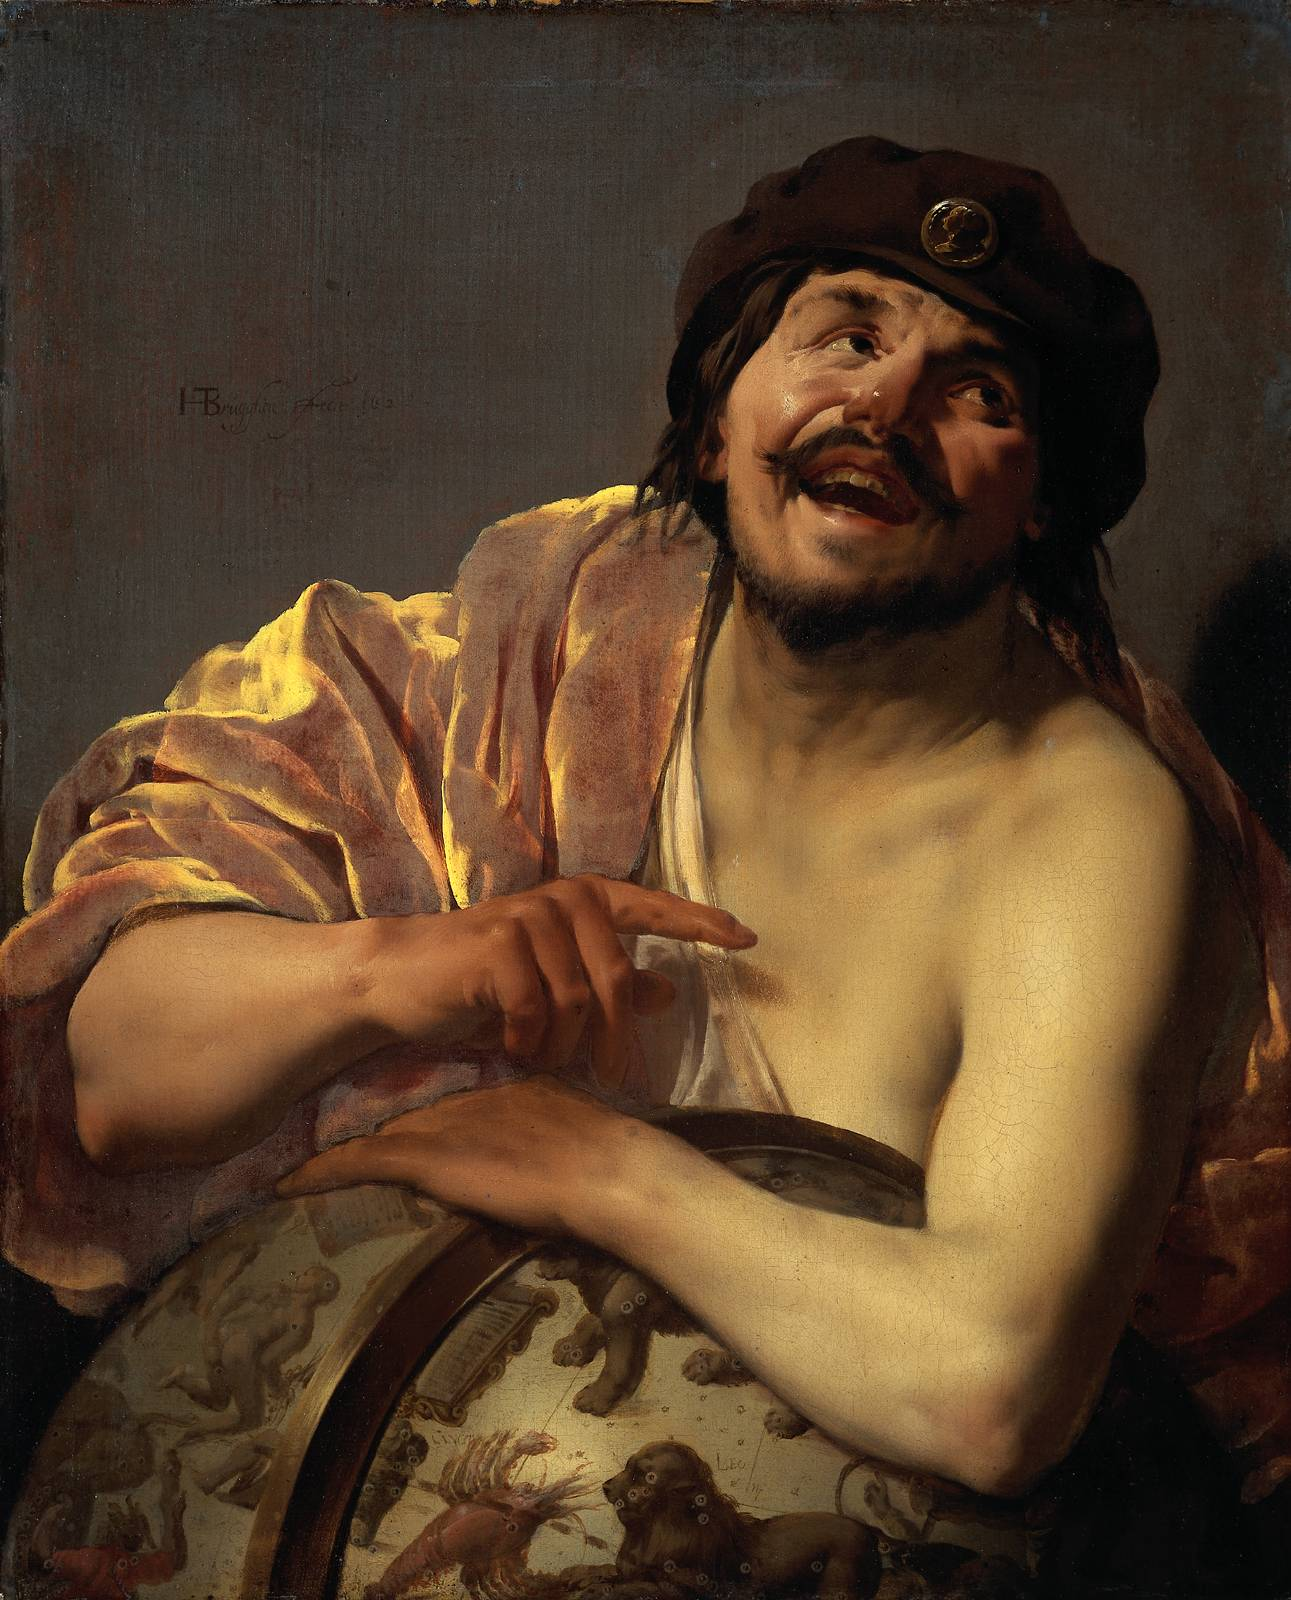
\includegraphics[width=0.4\linewidth]{../Chapter2/fig/democritus.jpg}
		\caption{Democritus}
		\label{fig:democritus}
	\end{subfigure}
	\caption{ Two greek philosophers, who made important philosophical
		contributions our understanding of matter. Empedocles (left), postulated the
		precursor to the elemental theory of matter ~\needcite{} and Democritus
		(right), postulated the precursor to the atomic theory of matter.  }
	\label{fig:atomists}
\end{figure}

Democritus was part of a movement of thought which was first to make the
intellectual jump that perhaps matter was not a continuum, but instead, composed
of 'atomon', small, indivisble particles which when configured togehter, created
all that is observable ~\needcite{}. Empedocles was making equally important
philosophical strides - in a manner complimentary to Democrits' opinion that
matter must be made of atomon, Empedocles argued that matter is composed of
elemental primatives ~\needcite{}.

Although Empedocles' 'periodic table' was only composed of Earth, Water, Fire,
and Air, the idea that some unseen transmutation of elemental forces might
generate observables in nature with quite different (but perhaps reminiscent)
properties then the 'pure substances' was an important step forward.
Proto-scientists were beginning to generate models which derived our complicated
observations, from simpler forms.

It took centuries of cultivation, leading up to the Scientific Revolution, for
the next great steps to occur, for science. Thankfully, the luminaries of the
Islamic Golden Age kept the fires of inqury burning ~\needcite{}.

\subsection{The Scientific Revolution}

Thanks to the mathematical foundations laid out, build, and maintained by the
minds of the Islamic Golden Age, Europe was well poised to reignite the flames
of scientific inquiry, during the post Renaissance Scientific Revolution
~\needcite{}.

This period of growth in science was unprecidented during the Scientific
Revolution, thanks to the seeds of empiricism germinated during the Islamic
Golden Age, fertilized by the Italian Renaissance, and helped to flourish
through British Empricism ~\needcite{}.

\begin{figure}[ht]
	\centering
	\begin{subfigure}{.5\textwidth}
		\centering
		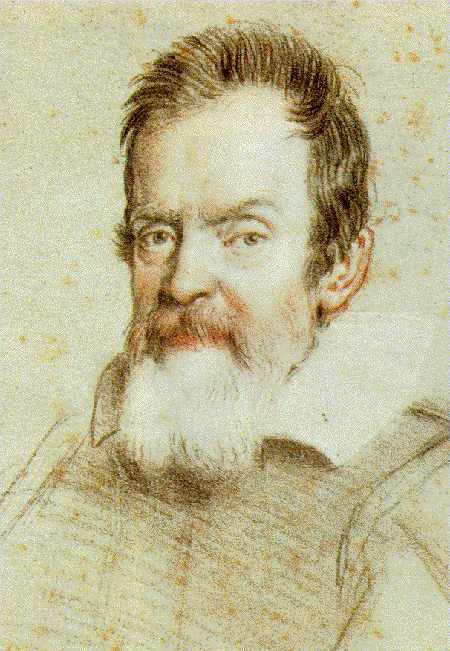
\includegraphics[width=0.4\linewidth]{../Chapter2/fig/galileo.jpg}
		\caption{Galileo}
		\label{fig:galileo}
	\end{subfigure}%
	\begin{subfigure}{0.5\textwidth}
		\centering
		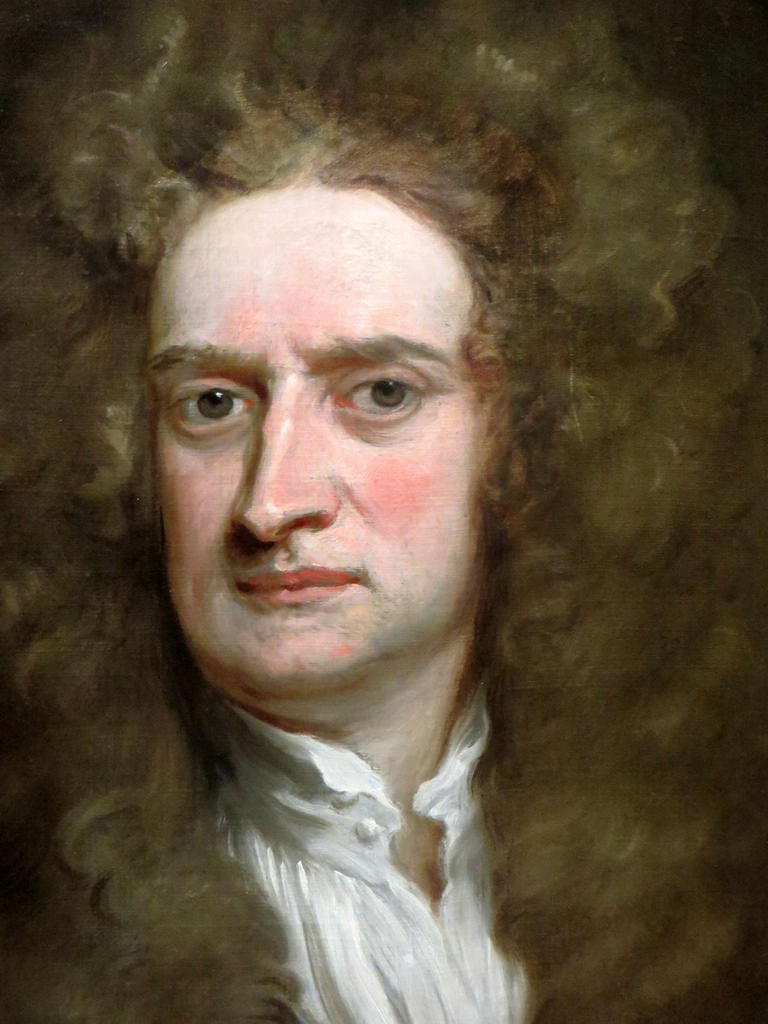
\includegraphics[width=0.4\linewidth]{../Chapter2/fig/newton.jpg}
		\caption{Newton}
		\label{fig:newton}
	\end{subfigure}
	\caption{ 
		Giants in the age of Empiricism, Newton (left) and
		Galileo (right) both made foundational contributions to Physics.
		Galileo lived in Italy, born in 1564 and dying in 1642. Newton lived in
		England from 1642 until his death in 1727
	}
	\label{fig:newtongalileo}
\end{figure}

\subsubsection{Galileo Galilei}
While Galileo is best known for his work in Observational Astronomy, his
importance to science extends beyond this. During his years in exile for his
controversial views of the heliocentric universe, he produced some of his most
important scientific work in kinematics ~\needcite{}. What made this work
remarkable is the care that Galileo took in merging careful mathematical
modeling with well designed experimentation. This methodical approach to inquiry
laid the foundation for others to slowly begin to pull back the curtains
obscuring physical law.

Galileo's formalization of the scientific method inexorably set science on a
course to delving deep into the nature of matter, and the laws of nature.

\subsubsection{Isaac Newton}
Fittingly born in the same year as Galileo's death, Isaac Newton would carry on
Galileo's legacy of rigorous mathematical modeling mixed with experimentaiton.
Perhaps no other scientist has touched so many different aspects of physics,
from theories of propegation of light, to celestial mechanics, to mathematics,
and kinematics.

Newton's Principia is perhaps the most important scientific work ever published.
It opened the doors of the universe in a way that nobody has since duplicated.
Newtons' laws of motion are still taught in school today, and although they have
since been shown to be inaccurate at the smallest and largest scales, they still
provide startlingly accurate predictions for the regular motion of matter.

One particularly tantelizing theory of Newton's was the corpuscular theory of
light. Although not his most influential theory by far, the idea that an
apparently continuous medium such as a beam of light might be made of small
packets of energy (corpuscules) turned out to be partially right ~\needcite{}.

Newton's theories, and contributions to science are enormous, and have moved us
deeper still into the underpinnings of matter. It would not be until roughly 200
years after his death, in the 19th century, that we finally can take the first
steps into the world of the atomic, and sub-atomic: the world of the proton. 

\subsection{Atomic Theory}

On the shoulders of giants such as Newton and Gallileo, science finally came to
know the tool which has been indispensable to modern particle physics:
scattering. Rutherford and Thompson both carried out the most important
scattering experiments in modern science, and provided us with the first hints
of a hidden, quantum world, though it would not be until the 20th century that
these important experiments would be fully contextualized with a theory of
quantum scattering.

Scattering experiments offer a very powerful method where we one uses a well
known initial state of matter (typically in the form of a beam), allows this
beam to interact with an unknown configuration of matter, and measures the
scattered beam. By carefully studying the kinematics of the scattered beam, we
can create models which allow us to understand the structure of the target
matter or describe the nature of the interaction between the beam and target. 

\begin{figure}[ht]
	\centering
	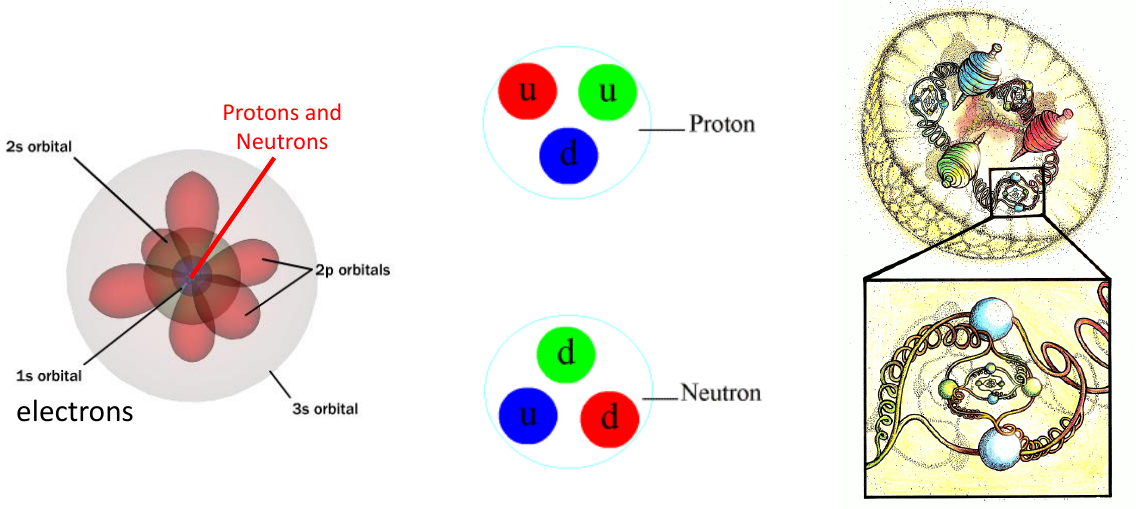
\includegraphics[width=\linewidth]{../Chapter2/fig/scale_of_matter.png}
	\caption{
		As we journey down further in scale, matter begins to look quite different.
		In fact, the models we use are scale dependant.
		Thomson~\ref{fig:thomsonrays}, and Rutherford~\ref{fig:rutherford} began to
		see matter as collections of atoms (left), though it would not be until 20th
		century quatum mechanics that electron orbitals were discovered. Soon,
		nuclei were discovered to be divisible into protons an neutrons (center),
		which in turn were discovered to be composed of a sea of quarks and gluons
		(right). (Right image drawn by the talented Astrid Morreale, PhD)
	}
	\label{fig:scale_of_matter}
\end{figure}

\subsubsection{John Dalton}

While many had postulated the existance of atoms, the first evidence based
theory which suggested the existance of atoms was produced by John Dalton in the
early 19th century. Dalton made an important conceptual leap to relate the
existance of stoicheometric ratios in chemistry to the presence of small,
individual funcitonal units in his experiements with chemical reactions.
Dalton's realization was only made possible due to his careful accounting of
reactants in his experiments.

It was not until Einstein's 1905 theory on Brownian Motion was experimentally
verified by Jean Perrin to place limits on the mass and size of atoms that
Dalton's atomic theory was ultimately vindicated~\cite{Patterson200750}.

\subsubsection{J.J. Thompson}

\begin{figure}[ht]
	\centering
	\begin{subfigure}{.4\textwidth}
		\centering
		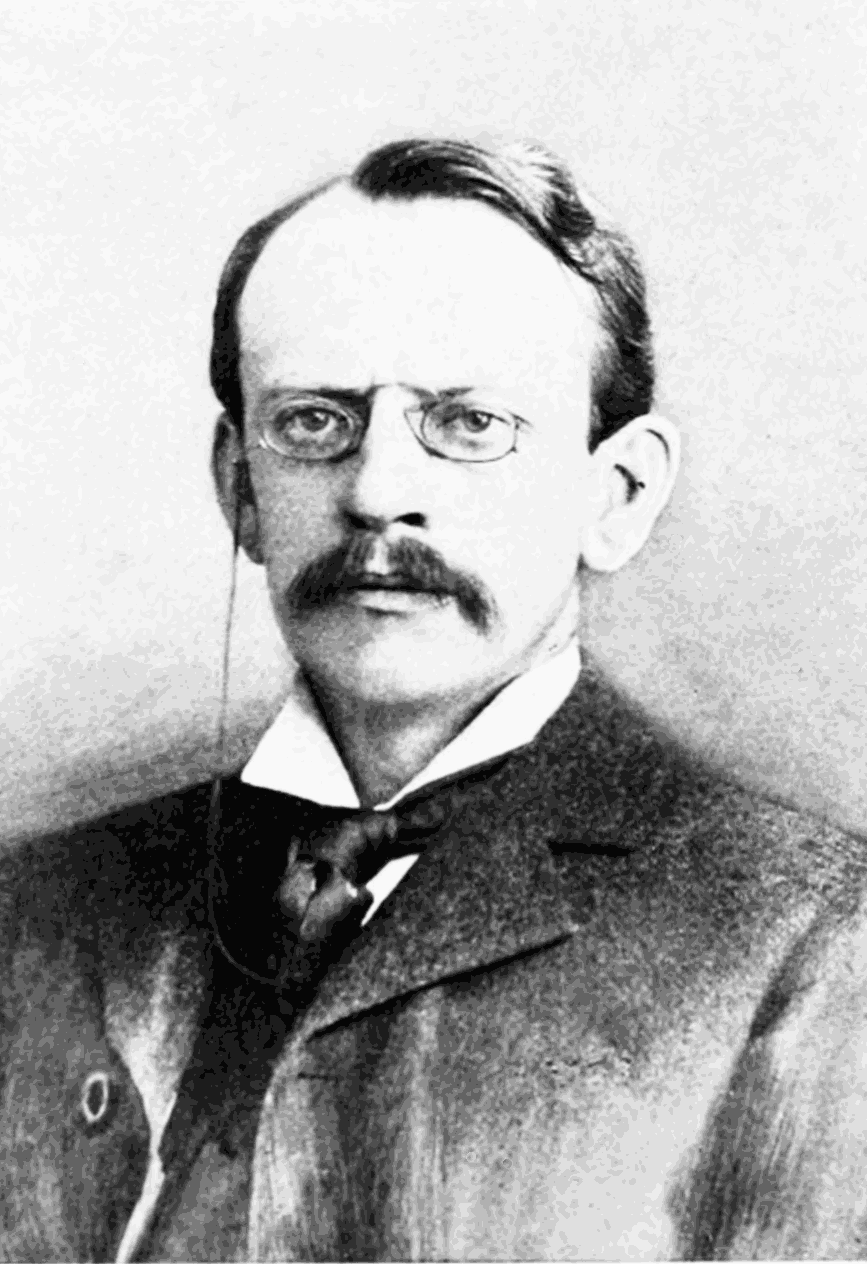
\includegraphics[width=0.4\linewidth]{../Chapter2/fig/jjthomson.png}
		\caption{J.J. Thomson}
		\label{fig:thomsonportrait}
	\end{subfigure}%
	\begin{subfigure}{0.6\textwidth}
		\centering
		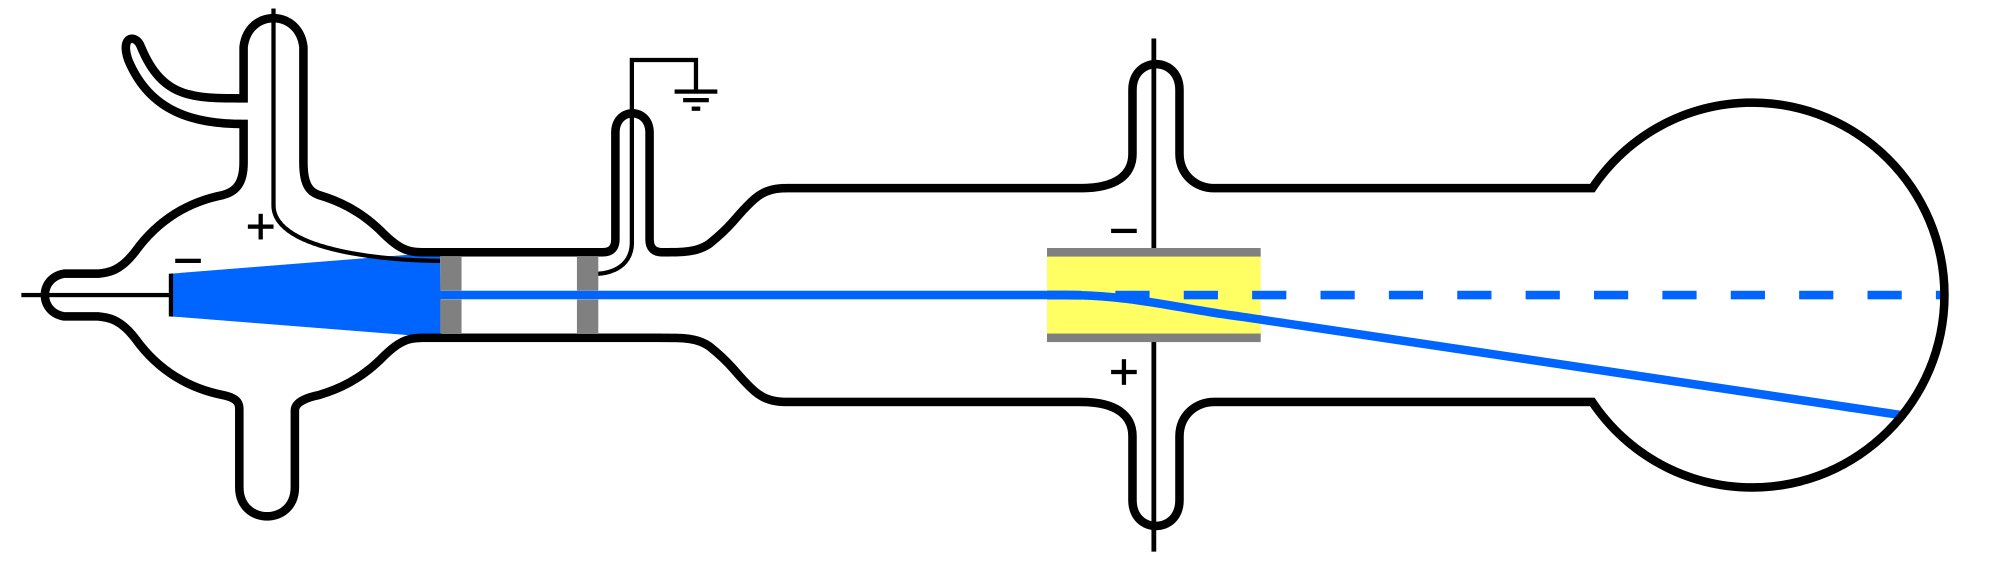
\includegraphics[width=0.4\linewidth]{../Chapter2/fig/cathoderaytube.png}
		\caption{Cathode Ray Tube}
		\label{fig:thomsoncathode}
	\end{subfigure}
	\caption{ 
		Left: J.J. Thomson, who showed that cathod ray tubes were in fact producing
		the first observed subatomic particle: the electron. Right: A cartoon of
		Thomson's cathod ray tube setup. Electrons would be deflected by a magnetic
		field, sent from cathode to anode.
	}
	\label{fig:jjthomson}
\end{figure}

Thomson (Figure~\ref{fig:jjthomson}) would discover that atoms are not the
smallest, indivisible piece of matter. In his landmark experiment, he used
cathode ray scattering experiments to show that cathode rays were in fact
subatomic particles. He showed these cathode rays were identical to particles
given off by the photoelectric effect, and that these same particles were
responsible for electric current. He had discovered the electron. And, if atoms
were not the smallest piece of matter, then perhaps, atoms themselves might not
be 'indivisible' as previously thought~\cite{nobelthomson2014}.


\subsubsection{Ernest Rutherford}

\begin{figure}[ht]
	\centering
	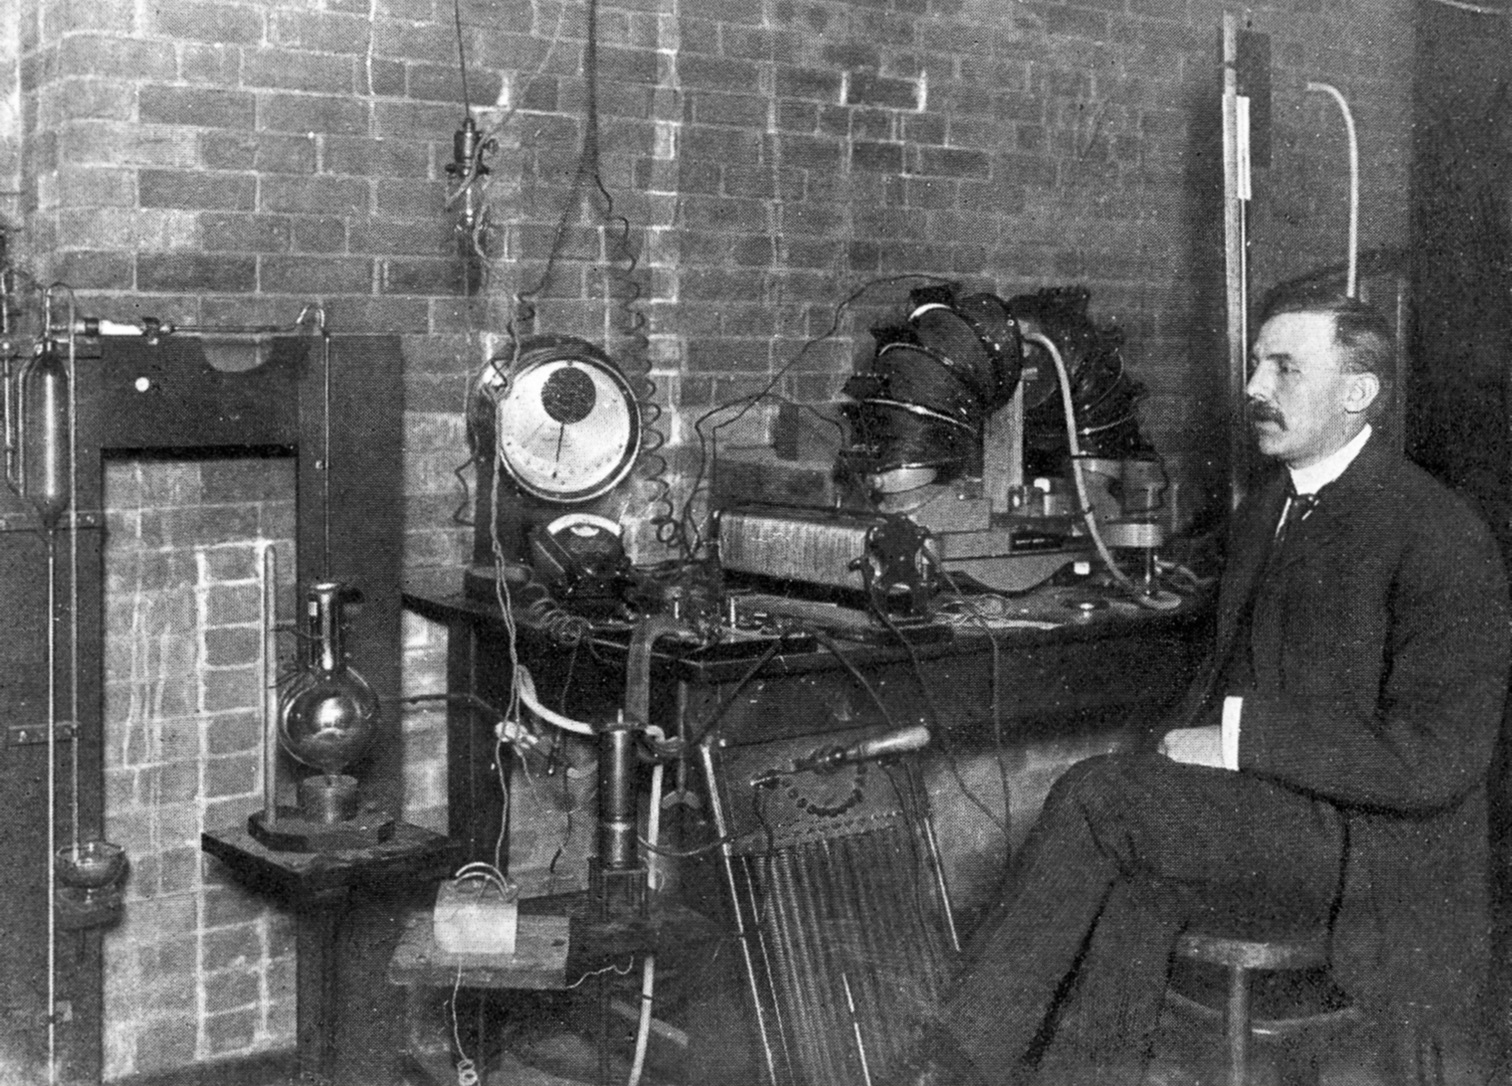
\includegraphics[width=0.6\linewidth]{../Chapter2/fig/ernestrutherford.jpg}
	\caption{Ernest Rutherford, in his lab.}
	\label{fig:rutherford}
\end{figure}

Ernest Rutherford (Fig~\ref{fig:rutherford}) was the first to show that atoms
themselves were highly structured - and consisted of a small dense center, later
called the nucleus.

\begin{figure}[ht]
	\centering
	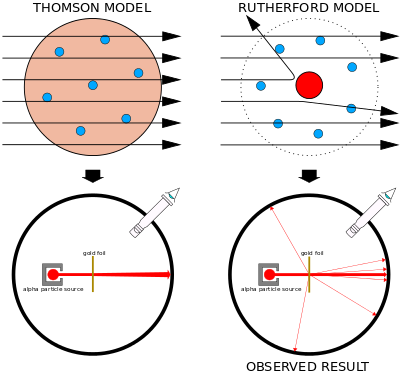
\includegraphics[width=0.6\linewidth]{../Chapter2/fig/geiger_marsden.png}
	\caption{
		Ernest Rutherford's historic experiment, showing (top right) that atoms were
		composed of a small dense nucleus, in contrast to Thomson's 'pudding model'
		of homogenous charge (top left). The experiment, (bottom left and right)
		contrast the expected results (bottom left) against the observed results
		(bottom right).
	}
	\label{fig:geigermarsden}
\end{figure}

Rutherford's work with radioactivity was of fundamental importance, he
discovered and classified both alpha-particle radioactivity and beta-particle
radioactivity. Further studies into these types of nuclear radiation would
unlock the nucleus of atoms through the work of future scientists. Notably,
Rutherford disovered the proton.

Rutherford's proposed planetary model for the nucleus, while technically wrong,
shifted paradigmns from continus atoms, to the more familiar nuclus + electron
cloud model which has been spectacularly modeled and verified with the
forthcoming scientists which defined the field of quantum mechanics.

Rutherford's work helped push us our of the cocoon of classical mechanics into
the weird world of the quantum mechanics - scientists would soon find that the
nucleus is not just a dense concentration of charge, but a probabalistic
structure, with rich subnuclear structure.

\subsection{Modern Origins}

\subsubsection{Quantum Mechanics}

During Rutherford's time, experiments were already underway which were
investigating modeling light as a wave phenomena. This was in contrast to
Newton's (unverified) corpuscular theory of light. The argument whether light
was wave-like or partilce-like eventually lead to a classical field theory
describing light, and the electromagnetic interaction, yet scientist such as Max
Plank were proposing theories which required the quantization of light.
~\needcite{}. Einstein would show that in his analysis of the photoelectric
effect, that light indeed was quantized into 'corpuscules'. The naiscent atomic
theory of matter was also hinting at a hidden, quantized world.

\begin{figure}
	\centering
	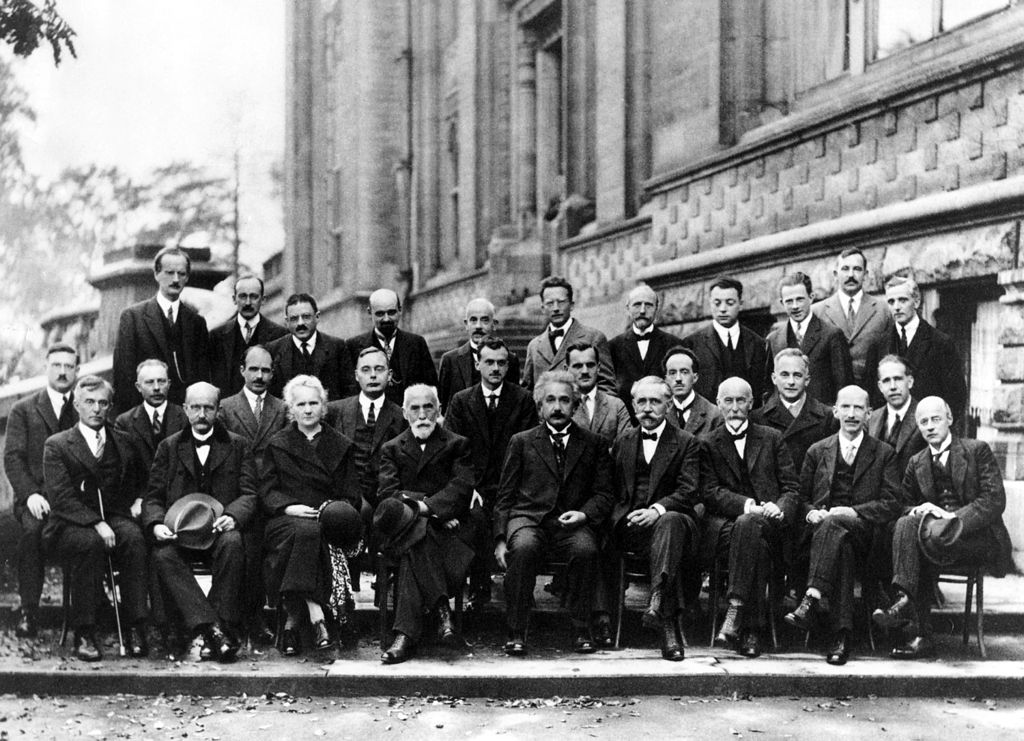
\includegraphics[width=0.7\linewidth]{../Chapter2/fig/solvay.jpg}
	\caption{
		The attendees of the Solvay Conference in Brussles, 1927.
	}
	\label{fig:solvay}
\end{figure}

At the Solvay Conference in Brussles, Figure~\ref{fig:solvay}, in 1927, we saw
an unprecidented gathering of some of the most important figures in modern
physics, all in one place, laying down the foundations of what would become
quantum mechanics. These scientists defined the nature and rules of quantum
mechanics - the weird model which accomodates a duality of matter - both
wave-like, and particle like. The notion that probing the sturcture of matter
did not yield a simple, deterministic hierarchy of strucutre was revolutionary,
confusing, and bizarre, and still is to this day.

It was found that not only light posesses this wave-particle duality, but also
the very particles that make up atoms as well. These models were formalized by
Dirac, Hilbert and von Neumann ~\needcite{}.

\subsubsection{Quantum Electrodynamics}

Though experiment tended to lead theory, regarding understanding the composition
and rules of interactions in matter, in the mid 20th century, further
refinements and additions to quantum mechanics gave birth to quantum field
theory. While early quantum models were very successful at describing static
particles trapped in static potentials - such as refining atomic theory to
include predicitions of observed atomic spectra, more work was needed to
understand the relationship between electrical currents, light and magnetism.
These concepts were all related by Maxwell ~\needcite{} in the latter half of
the 19th century, but did not make good predictions for systems in motion.

Dirac was first to create a model for describing the electron, its behavior in
electromagnetic fields, and photon emission and absorption, under fully
relativistic and quantum conditions~\needcite{}. Dirac's model was so
successful, that it would become the basis for what we now call quantum
electrondynamics. Much of the mathematical formalism has been reused to describe
other field theories, which are the ultimate language which model and describe
the structure of matter - including the insides of a proton. 

\begin{figure}[ht]
	\centering
	\begin{subfigure}{.4\textwidth}
		\centering
		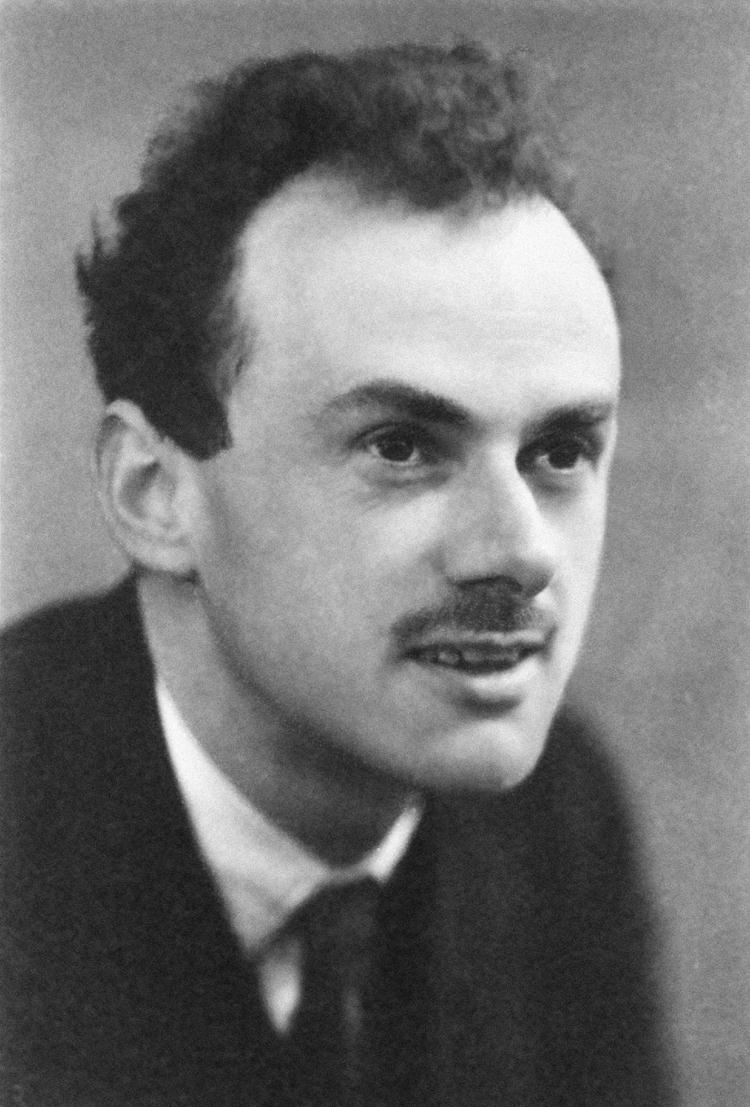
\includegraphics[width=0.4\linewidth]{../Chapter2/fig/pauldirac.jpg}
		\caption{Paul Dirac, 1933}
		\label{fig:pauldirac}
	\end{subfigure}%
	\begin{subfigure}{0.6\textwidth}
		\centering
		\begin{equation}
			\left(\beta mc^2 + c\left(\sum_{n \mathop =1}^{3}\alpha_n p_n\right)\right) \psi (x,t) = i \hbar \frac{\partial\psi(x,t) }{\partial t}
		\end{equation}
		\caption{The Dirac Equation}
		\label{eq:diracquation}
	\end{subfigure}
	\caption{ 
		Paul Dirac, next to his original formulation of the Dirac Equation,
		describing the wave function for an electron with rest-mass m, in terms of
		its spacetime coordinates.
	}
	\label{fig:thomsonrays}
\end{figure}

Dirac's work also began to incorporate relativistic effects in his wave
equations modeling the electron, as well as crucially incorporating the spin
(i.e. Dirac Spinors) of these particles, which were important for making precise
predictions for atomic spectra~\needcite{}.

By this time, the proton was already known to reside in the enigmatic nucleus of
atoms, however, attempts to use Quantum Electrodynmics to describe the state of
the nucleus failed - it was clear that there was a very strong force, holding
together the protons of a nucleus tightly - far in excess of the electromagnetic
repulsion felt by the positively charged particles. There was a completely
different coupling strength between this apparent strong nuclear force, and the
better known electromagnetic coupling. Further complicating an understanding of
the nucleus is the fact that as the length scale of probing decreases, the
energies probed increase, fundamentally making the nucleus a relativistic
object. Experimental physics would once again, forge ahead, in attempting to
understand the inner workings of the nucleus, in the time-honored tradition of
performing scattering experiments.

\clearpage
\subsubsection{Quantum Chromodynamics}

The hydrogen atom, and its spectra was well modeled with quantum mechancis by
the end of early 20th century, however attempts to study Helium were not as
successful ~\needcite{}. However, in 1932,  when Chadwick turned a beam of
helium particles (at that time only known as $\alpha$ particles) on a sample of
Beryllium, he observed that neutral, non-ionizing, penetrating radtition was
produced ~\cite{KraussParticleHistory}. Photons were ruled out as possible
candidates, leading to the discovery of the neutron. Protons and neutrons were
hypothesized by Heisenberg to both be the same state of a new conceptual
particle, the nucleon, ~\cite{Heisenberg1952}. In the same year, Anderson
discovered the positron. 

By 1934, Hideki Yukawa (Fig.~\ref{fig:hidekiyukawa}) had created an effective
field theory for interactions of 'elementary particles' (at this time, thought
to be protons and neutrons). He predicted the existence of mesons, and wrote
down an effective field theory which described how protons and neutrons bind
together in the nucleus~\cite{Yukawa1935}. 

Though non-relativistic quantum mechanics was mostly complete by 1934,
scientists were already hard at work incorporating relativistic corrections to
the theory. Experiments with cosmic rays soon revealed the existance of muons
and the first observation of mesons.

\begin{figure}[ht]
	\begin{center}
		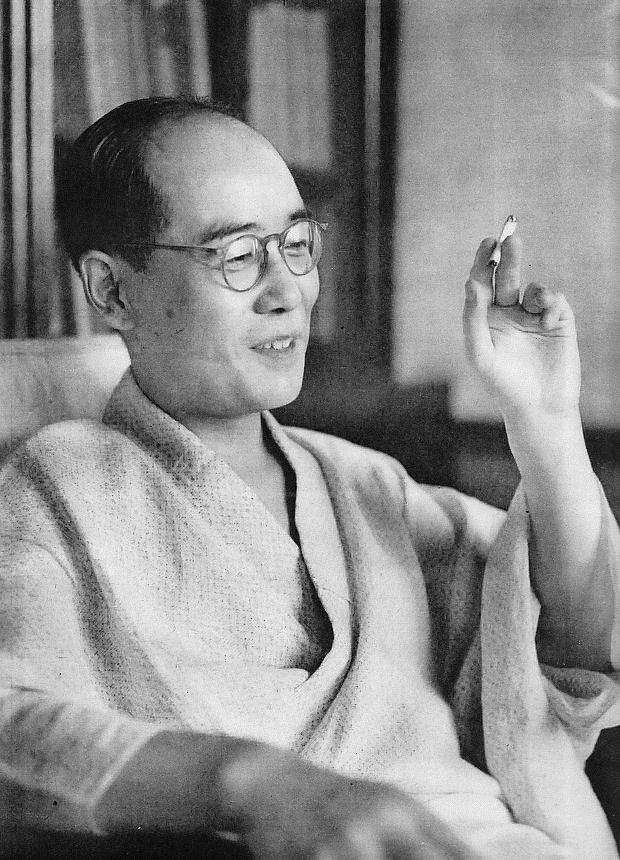
\includegraphics[width=0.5\linewidth]{../Chapter2/fig/hidekiyukawa.jpg}
	\caption{
		Hideki Yukawa, the first Japanese Nobel Laurate and publisher of influential
		research on the theory of mesons, and other elementary particles.
	}
	\label{fig:hidekiyukawa}
\end{center}
\end{figure}

Three separate paths eventually lead to the development of particle
accellerators, which are to date, the best mechanism we possess in physics to
probe nuclear structure. These accelerators are an outgrowth
of ever more intense Rutherford-style experiments, Tandem Van-Der-Graaf
generators, resonant acceleration techniques, RF lineacs, and betatron
accelerators~\cite{Bryant1994}.

By the 1950s, a cornecopia of strange new particles had been discovered, both
matter and antimatter. But scientists drove forward, deeper, yearning to
discover what was fundamental. By the 50's, neutrinos had been proposed, as well
as Kaons, Pions, and Lambdas. Physicists were doing nuclear chemistry, in a
sense, attempting to work out how quickly some particles decayed, and what
decays were allowed or forbidden - scinece entered an age of nuclear alchemy.

"Strange" particles were discovered ($K$ and $\Lambda$), so called because in
bevatron experiments, they were produced in great quantities, but were slow to
decay, unlike the faster $\pi$ decay. Gell-Mann proposed that this strangeness
in matter was due to a new quantum number (he called it 'strangeness'). The name
stuck.
~\cite{Gell-Mann1953},~\cite{Gell-Mann1956},~\cite{KraussParticleHistory}.


Gell-Mann (8 fold way) Feynman, Wilczek, Weinberg, T Hooft, DGLAP. David Gross

Although Gell-Mann's simple quark model of baryons ~\needcite{} predicts the
correct quantiy for the spin of the proton, the work of Ashman et al (1988)
~\needcite{} at the European Muon Collaboraiton directly measured a portion of
the proton sturcture function $g_1$ and found that a rather small fraction of
the prton spin comes from quarks - and most of the spin is carried by the
gluons (Figure~\ref{fig:emc_g1_result}).

\begin{figure}[ht]
	\begin{center}
	
\includegraphics[width=0.5\linewidth]{../filler/squareimg.png}
	\caption{~\needfig{} ~\needcap{}. Results of EMC experiment showing that the structure
	function g1, tells us a thing about proton spin.}
	\label{fig:emc_g1_result}
\end{center}
\end{figure}

\subsubsection{Proton Spin Crisis}

\clearpage
\section{How to Model Proton Spin}
\subsection{ structure functions}
\subsection{ proton spin decomposition}
\subsection{ unpolarized parton distribution functions}
\subsection{ polarized parton distribution functions}
\subsection{ that sweet table from Delia hasch}
\subsection{ discussion $\bar{q}$, $q$, $L_q$, $g$}
\subsection{ DSSV }

\clearpage
\section{How to Measure Proton Spin}
\subsection{ physics probes for proton spin}
\subsection{ W cross section}
\subsection{ derivation of Asymmetry}
\subsection{ kinematic extremes of Asymmetry}

\clearpage
\section{Experimental Findings in Proton Structure}
\subsection{Summary of Data on Structure Functions}
\subsection{CERN}
\subsection{ZEUS}
\subsection{HERA}
\subsection{HERMES}
\subsection{COMPASS}
\subsection{EMC}
\subsection{SLAC}
\subsection{JLAB}

\clearpage
\section{Cross Sections and Luminosity}
\begin{itemize}
		\item vernier analysis note intro, equations
		\item summarize the papers on Lumoninosity
\end{itemize}

\clearpage
